% THIS IS SIGPROC-SP.TEX - VERSION 3.1
% WORKS WITH V3.2SP OF ACM_PROC_ARTICLE-SP.CLS
% APRIL 2009
%
% It is an example file showing how to use the 'acm_proc_article-sp.cls' V3.2SP
% LaTeX2e document class file for Conference Proceedings submissions.
% ----------------------------------------------------------------------------------------------------------------
% This .tex file (and associated .cls V3.2SP) *DOES NOT* produce:
%       1) The Permission Statement
%       2) The Conference (location) Info information
%       3) The Copyright Line with ACM data
%       4) Page numbering
% ---------------------------------------------------------------------------------------------------------------
% It is an example which *does* use the .bib file (from which the .bbl file
% is produced).
% REMEMBER HOWEVER: After having produced the .bbl file,
% and prior to final submission,
% you need to 'insert'  your .bbl file into your source .tex file so as to provide
% ONE 'self-contained' source file.
%
% Questions regarding SIGS should be sent to
% Adrienne Griscti ---> griscti@acm.org
%
% Questions/suggestions regarding the guidelines, .tex and .cls files, etc. to
% Gerald Murray ---> murray@hq.acm.org
%
% For tracking purposes - this is V3.1SP - APRIL 2009

\documentclass{acm_proc_article-sp}
%\documentclass{sig-alternate}
\usepackage[numbers, sort, compress]{natbib}
\usepackage{xspace}
\usepackage{color}
\usepackage[usenames,dvipsnames]{xcolor}
%\usepackage{hyperref}
%\usepackage{mdwlist}
\usepackage{url}
\usepackage{subfigure}
%\usepackage{hyphenation}
\hyphenation{Map-Reduce}
\hyphenation{Ha-doop}
\usepackage{listings} 
\usepackage{enumerate}
\usepackage{paralist}

\newif\ifdraft
%\drafttrue
\ifdraft

\newcommand{\terminology}[1]{ {\textcolor{red} {(Terminology used: \textbf{#1}) }}}
\newcommand{\jhanote}[1]{ {\textcolor{red} { ***SJ: #1 }}}
\newcommand{\alnote}[1]{ {\textcolor{blue} { ***andreL: #1 }}}
\newcommand{\pnote}[1]{ {\textcolor{magenta} { ***pradeep: #1 }}}
\newcommand{\secrev}[1]{ {\textcolor{Bittersweet} { ***reviewer2: #1 }}}
\newcommand{\thirdrev}[1]{ {\textcolor{Bittersweet} { ***reviewer3: #1 }}}
\newcommand{\note}[1]{ {\textcolor{red} { ***Note: #1 }}}
\else
\newcommand{\terminology}[1]{}
\newcommand{\alnote}[1]{}
\newcommand{\pnote}[1]{}
\newcommand{\jhanote}[1]{}
\newcommand{\note}[1]{}
\fi

\newcommand{\up}{\vspace*{-1em}}
\newcommand{\upp}{\vspace*{-0.5em}}


\newcommand{\pilot}{Pilot\xspace}
\newcommand{\pilots}{Pilots\xspace}
\newcommand{\pilotjob}{Pilot-Job\xspace}
\newcommand{\pilotjobs}{Pilot-Jobs\xspace}
\newcommand{\pilotcompute}{Pilot-Compute\xspace}
\newcommand{\pilotcomputes}{Pilot-Computes\xspace}
\newcommand{\pilotmapreduce}{Pilot-MapReduce\xspace}
\newcommand{\mrmg}{MR-Manager\xspace}
\newcommand{\computeunit}{Compute Unit\xspace}
\newcommand{\computeunits}{Compute Units\xspace}
\newcommand{\cu}{CU\xspace}
\newcommand{\cus}{CUs\xspace}
\newcommand{\cs}{Compute Service\xspace}
\newcommand{\css}{Compute Services\xspace}
\newcommand{\pcs}{Pilot Compute Service\xspace}
\newcommand{\dataunit}{Data Unit\xspace}
\newcommand{\dataunits}{Data Units\xspace}
\newcommand{\du}{DU\xspace}
\newcommand{\dus}{DUs\xspace}
\newcommand{\pilotdata}{Pilot-Data\xspace}
\newcommand{\pd}{PD\xspace}
\newcommand{\pds}{Pilot Data Service\xspace}
\newcommand{\pdss}{Pilot Data Services\xspace}
\newcommand{\su}{SU\xspace}
\newcommand{\sus}{SUs\xspace}
\newcommand{\schedulableunit}{Schedulable Unit\xspace}
\newcommand{\schedulableunits}{Schedulable Units\xspace}
\begin{document}

\conferenceinfo{MapReduce'12,} {June 18-19, 2012, Delft, The Netherlands.} 
\CopyrightYear{2012} 
\crdata{978-1-4503-1343-8/12/06} 
\clubpenalty=10000 
\widowpenalty = 10000

%\title{An Extensible Pilot-based MapReduce Implementation}

\title{Pilot-MapReduce: An Extensible and Flexible
  MapReduce Implementation for Distributed Data}

%
% You need the command \numberofauthors to handle the 'placement
% and alignment' of the authors beneath the title.
%
% For aesthetic reasons, we recommend 'three authors at a time'
% i.e. three 'name/affiliation blocks' be placed beneath the title.
%
% NOTE: You are NOT restricted in how many 'rows' of
% "name/affiliations" may appear. We just ask that you restrict
% the number of 'columns' to three.
%
% Because of the available 'opening page real-estate'
% we ask you to refrain from putting more than six authors
% (two rows with three columns) beneath the article title.
% More than six makes the first-page appear very cluttered indeed.
%
% Use the \alignauthor commands to handle the names
% and affiliations for an 'aesthetic maximum' of six authors.
% Add names, affiliations, addresses for
% the seventh etc. author(s) as the argument for the
% \additionalauthors command.
% These 'additional authors' will be output/set for you
% without further effort on your part as the last section in
% the body of your article BEFORE References or any Appendices.

\numberofauthors{3} %  in this sample file, there are a *total*
% of EIGHT authors. SIX appear on the 'first-page' (for formatting
% reasons) and the remaining two appear in the \additionalauthors section.
%
\author{
% You can go ahead and credit any number of authors here,
% e.g. one 'row of three' or two rows (consisting of one row of three
% and a second row of one, two or three).
%
% The command \alignauthor (no curly braces needed) should
% precede each author name, affiliation/snail-mail address and
% e-mail address. Additionally, tag each line of
% affiliation/address with \affaddr, and tag the
% e-mail address with \email.
%
\alignauthor Pradeep Kumar Mantha\\
       \affaddr{Center for Computation and Technology}\\
       \affaddr{Louisiana State University}\\
       \affaddr{216 Johnston}\\
       \affaddr{Baton Rouge, LA}
       \email{pmanth2@cct.lsu.edu}
\alignauthor Andre Luckow\\
       \affaddr{Center for Computation and Technology}\\
       \affaddr{Louisiana State University}\\
       \affaddr{216 Johnston}\\
       \affaddr{Baton Rouge, LA}
       \email{aluckow@cct.lsu.edu} 
\alignauthor Shantenu Jha\\
      \affaddr{Center for Autonomic Computing}\\
     \affaddr{Rutgers University}\\
      \affaddr{94 Brett Road}\\
      \affaddr{Piscataway, NJ}
     \email{shantenu.jha@rutgers.edu}
}
% There's nothing stopping you putting the seventh, eighth, etc.
% author on the opening page (as the 'third row') but we ask,
% for aesthetic reasons that you place these 'additional authors'
% in the \additional authors block, viz.
% \additionalauthors{Additional authors: John Smith (The Th{\o}rv{\"a}ld Group,
% email: {\texttt{jsmith@affiliation.org}}) and Julius P.~Kumquat
% (The Kumquat Consortium, email: {\texttt{jpkumquat@consortium.net}}).}
\date{30 July 1999}
% Just remember to make sure that the TOTAL number of authors
% is the number that will appear on the first page PLUS the
% number that will appear in the \additionalauthors section.

%thus the ability to analyze data by localizing it will yield limited
%returns.

\maketitle
\begin{abstract}
  The volume and complexity of data that must be analyzed in
  scientific applications is increasing exponentially. Often, this
  data is distributed, thus efficient processing of large distributed
  datasets is required, whilst ideally not introducing fundamentally
  new programming models or methods. For example, extending MapReduce
  -- a proven and effective programming model for processing large
  datasets -- to work more effectively on distributed data and on
  different infrastructure %(such as non-Hadoop, general-purpose
                           %clusters)
  is desirable. MapReduce on distributed data requires effective
  distributed coordination of computation (map and reduce) and data,
  as well as distributed data management (in particular the transfer
  of intermediate data). We posit that this can be achieved with an
  effective and efficient runtime environment and without refactoring
  MapReduce itself.  To address these requirements, we design and
  implement \pilotmapreduce (PMR) -- a flexible,
  infrastructure-indepen\-dent runtime environment for MapReduce.  PMR
  is based on \pilot abstractions for both compute (Pilot-Jobs) and
  data (Pilot-Data): it utilizes Pilot-Jobs to couple the map phase
  computation to the nearby source data, and Pilot-Data to move
  intermediate data using parallel data transfers to the reduce phase.
  We analyze the effectiveness of PMR on applications with different
  characteristics (e.\,g.\ different volumes of intermediate and
  output data).  We investigate the performance of PMR with
  distributed data using a Word Count and a genome sequencing
  application over different MapReduce configurations.  Our
  experimental evaluations show that the Pilot abstractions are
  powerful abstractions for distributed data: PMR can lower the
  execution time on distributed clusters and that it provides the
  desired flexibility in the deployment and configuration of MapReduce
  runs to address specific application characteristics.

%  both powerful and flexible in particular

%   and achieve an
%   optimal performance, both locally and over multiple clusters.

% We analyze the effectiveness of PMR for different applications based
% upon the ratio of data-aggregation between phases as well as single
% and hierarchical MapReduce.
\end{abstract}

%Hierarchical MapReduce is a potential distributed solution only for
%high data aggregation applications leaving single cluster-MapReduce as
%an optimal solution for zero or ballooning data applications~\cite
%{weissman-mr-11}, which is still costly as it involves initial huge
%data transfers of source data to the single cluster.

% A category with the (minimum) three required fields

%A category including the fourth, optional field follows...
\category{D.1.3}{Software}{Concurrent Programming-}{Distributed
  programming/parallel programming} 
\terms{Design, Experimentation, Performance}

 \keywords{ MapReduce, Distributed Computing, Pilot Job and Data, Simple API for Grid
  Applications (SAGA), Genome Sequence Alignment, BWA,}


%\keywords{Pilot-Jobs, MapReduce, Genome Sequencing}% NOT required for Proceedings
\upp
\section{Introduction}

%General Motivation

There are various challenges associated with processing of data at
extreme scales: which has become a critical factor in many science
disciplines, e.\,g.\ in the areas of fusion energy (ITER),
bioinformatics (metagenomics), climate (Earth System Grid), and
astronomy
(LSST)~\cite{Jha:2011fk}. The
volumes of data produced by these scientific applications is
increasing rapidly, driven by advanced technologies (e.\,g.\
increasing compute capacity and higher resolution sensors) and
decreasing costs for computation, data acquisition and
storage~\cite{hey2009}. The number of applications that
either currently utilize, or need to utilize large volumes of
potentially distributed data is immense. The challenges faced by these
applications are interoperability, efficiently managing compute tasks,
and moving data to the scheduled compute location.

% which is inevitable in case of programming models like MapReduce.

%Intro to MapReduce
Processing large volumes of data is a challenging task. MapReduce is
an effective programming model for addressing this challenge.
MapReduce~\cite{Dean:2004:MSD:1251254.1251264} as originally developed
by Google aims to address the big data problem by providing an
easy-to-use abstraction for parallel data processing. The most
prominent framework for doing MapReduce computations is Apache
Hadoop~\cite{hadoop}. However, there are limitations to the current MR
implementations: (i) They lack a modular architecture, (ii) are
tied to specific infrastructure, e.\,g.\ Hadoop relies on the Hadoop
File System (HDFS), and (iii) do not provide efficient support for
dynamic and processing distributed data, e.\,g.\ Hadoop is designed
for cluster/local environment, but not for a high degree of
distribution.

% In particular when the source
% data and computing platform distributed widely, the most efficient
% architecture for processing data over the entire data set becomes non-trivial.
%Intro to weissman's MapReduce configurations and workload types.
%Why pilot abstractions

% as well as the limitations of existing MapReduce implementations, such
% as the limited support for distributed data. 

Pilot abstractions enable the clean separation of resource management
concerns and application/frameworks. In particular, \pilotjobs have
been notable in their ability to manage large numbers of compute units
across multiple high performance clusters, providing decoupling
application-level scheduling and system-level resource
management. But, there is also a need of an abstraction to liberate
applications from the challenging task of compute-data placement and
scheduling. The Pilot-API~\cite{pstar-2012} aims to address this issue
by providing a unified API for managing both compute and data
pilots. In this paper, we present \emph{BigData (BD)}, an extension of
the BigJob framework (BJ)~\cite{bigjob_web} to data. Both BigJob and
BigData provide a full implementation of the Pilot-API and enable the
management of resources, compute \& data units as well as the
relationships % \jhanote{what kind of relationship? haven't we already
%   introduced the notion of affinity?}
between them. Specifically, the
Pilot-API promotes affinities as a first class characteristic for
describing such relationships between compute and data elements and to
support dynamic decision making.

% Pilot-Data provides an abstraction
% for expressing and managing relationships between data units and/or compute
% units. The coupling of abstractions, Pilot-Jobs and Pilot-Data, provide a
% complete solution for data intensive applications to utilize distributed cyber
% infrastructure effectively. 

A critical aspect of MapReduce, is the management of data and compute
localities as well as the management of data movements, e.\,g.\
between the map and the reduce phase.  In this paper, we demonstrate
the efficient support of these capabilities via the Pilot
abstractions. We design and implement \pilotmapreduce \ -- a novel
\pilot-based MapReduce implementation which enables clean separation
of resource management and MapReduce application. We show how \pilot
abstractions are used for managing the map and reduce tasks and
intermediate shuffle data between them.  In addition, we show the
advantages of the \pilot-based architecture in terms of flexibility,
extensibility, scalability and performance; for example, we discuss
the usability of \pilot-abstractions in designing dynamic execution
workflows which involves multiple MapReduce computations.


Before we proceed further, it is critical to emphasize that it is not
the aim of this paper to suggest PMR as a replacement to Hadoop.
However, we posit that where MR-based applications need to be employed
over distributed data, including but not limited to clusters connected
over WAN, or production distributed cyberinfrastructure such as XSEDE,
EGI, PMR provides a flexible, extensible implementation of MR that is
also efficient.
 

This paper is organized as follows: Section~\ref{sec:related_work} presents
related works. Section~\ref{sec-pilot-impl} gives an overview of \pilot
abstractions and the BigData framework. In section~\ref{sec-pilot-mr} we discuss
the design and implementation of the \pilotmapreduce framework.
Section~\ref{sec-experiments} gives experiment setup and result analysis. The
conclusion and future work are given in Section~\ref{sec-conclusion}.

\upp\upp
% Introduction must lay out the fact that PMR does not as a
%   substitute Hadoop on dedicated clusters, but is useful on WAN
%   clusters and production infrastructure}

\section{Related Work}
\label{sec:related_work}
The MapReduce programming model~\cite{Dean:2004:MSD:1251254.1251264}
and the distributed file system (Google File System
(GFS)~\cite{Ghemawat:2003:GFS:1165389.945450}) were originally
pioneered by Google. Apache Hadoop~\cite{hadoop} is an open source
implementation of MapReduce. Hadoop also includes an implementation of
a distributed file system -- the Hadoop File System
(HDFS)~\cite{Borthakur:2007fk}. In addition the Hadoop ecosystems
includes several other projects, such as HBase (a system also inspired
by Google's BigTable), Hive, Pig and Zookeeper. The main limitation of
Hadoop MapReduce is that it forces applications into a very rigid
model. Hadoop e.\,g.\ is well suited for running a single MapReduce
application, but very limited in terms of extensibility, e.\,g.\ it
cannot efficiently run an ensemble of MapReduce simulations or support
a pipeline of multiple iterative MapReduce tasks. Also, the deployment
of Hadoop on HPC resources remains a challenge: the deployment in
user-space is complex and error-prone. Furthermore, MapReduce requires
the user to reload the data every time Hadoop is
initialized. \jhanote{Pradeep is the previous a property due to
  MapReduce in particular or is it true of Hadoop in general?} Also,
HPC resources often have shared distributed file system and only a
small amount of local storage, which leads to sub-optimal Hadoop
performance. Running Hadoop on multiple resources is in principal
possible, but firewall regulations often prohibit such deployment on
many infrastructures in practice.

% \thirdrev{1) it does not say specifically why HADOOP "is not suited" for distributed data. in fact we have seen HADOOP used for cross-data center deployments , which means longer network delays between parts of the cluster, and is indeed an example of *distributed* data. accordingly it does not highlight what it does specifically to overcome the potential disadvantages of HADOOP}
% \pnote{addressed in the above para} 

Sector/Sphere~\cite{Gu_Grossman_2009} is a parallel data processing
framework consisting of a distributed file system (Sector) and a data
processing engine (Sphere). In contrast to Hadoop, which operates on
file chunks, Sphere can execute arbitrary user-defined functions on a
stream of data.

Twister~\cite{Ekanayake:2010:TRI:1851476.1851593} is a 
MapReduce addressing particularly the requirement for supporting iterative 
MapReduce jobs. Twister allows the flexible composition of applications by 
specifying map and reduce tasks and the data flow between these tasks. 
Dryad~\cite{Isard:2007:DDD:1272998.1273005} provides distributed execution of
coarse-grain data-parallel applications. The entire execution is represented in
the form of data flow graphs, where the vertices represent the computational
tasks that can be paralleled on a set of computational resources and the links
between vertices tell Dryad what other vertices need to complete before a
particular vertex can start.

Several proposal for deploying MapReduce and Hadoop on distributed data and
resources exist: Weissman et\,al.~\cite{weissman-mr-11} explore different Hadoop
configurations to accommodate different distributed resource configurations. 
Qiu et\,al.~\cite{ecmls11-mr-autodock} also propose a hierarchical
MapReduce configuration that implements the Map-Reduce-Global Reduce pattern on 
top of distributed resources. 
% For management of the distributed data the implementation relies on GFarm~\cite{Mikami:2011:UGF:2082076.2082106}. 

SAGA-MapReduce~\cite{Sehgal:2011:UAI:1945091.1945329} is a SAGA-based
MapReduce implementation that utilizes the SAGA-API for accessing
system-level features, such as resource \& file management and
coordination. The SAGA-based approach enabled the decoupling of
infrastructure and application concerns enabling the support of a
wide-set of distributed infrastructure (e.\,g,\ grids and clouds). The
utilization of Pilot abstractions has several advantages compared to
the SAGA-only approach: (i) compute and data pilots allow an efficient
decoupling of resource allocation and usage, i.\,e.\ the MapReduce
master can efficiently schedule compute units containing mapper and
reduce tasks; (ii) the co-location of data and compute units can be
descriptively defined, and are automatically handled by Pilot
framework; this enables the applications to easily trade-off data
transfers and available compute capacities.

\pilotmapreduce utilizes \pilot abstractions for de-coupling the
MapReduce runtime, application-level scheduling and resource
management in order to provide a high degree of flexibility and
extensibility.

% In this paper, we  of \pilot-abstractions to design
% an infrastructure-independent runtime environment for MapReduce
% applications. 


% \jhanote{I realized that we don't formally reference hierarchical
%   mapreduce work -- Ref.~\cite{ecmls11-mr-autodock} in ECMLS'11 by
%   Judy Qiu et al}\alnote{done}

%data flow oriented frameworks


\upp
\section{Pilot Abstractions}
\label{sec-pilot-impl}


The P* model~\cite{pstar-2012} aims to provide a unified model for describing
and analyzing \pilotjob implementations. Figure~\ref{fig:figures_pstar} shows
the elements of the P* model. The P* model defines common elements of both
compute and data pilot implementations. Pilot abstractions for both compute and
data are the foundation of the \pilotmapreduce. In this section we give an
overview of the Pilot-API, which exposes the elements of the P* model to the
applications as well as the implementation of the BigJob and BigData framework.


\begin{figure}[t]
	\upp\upp
    \centering
    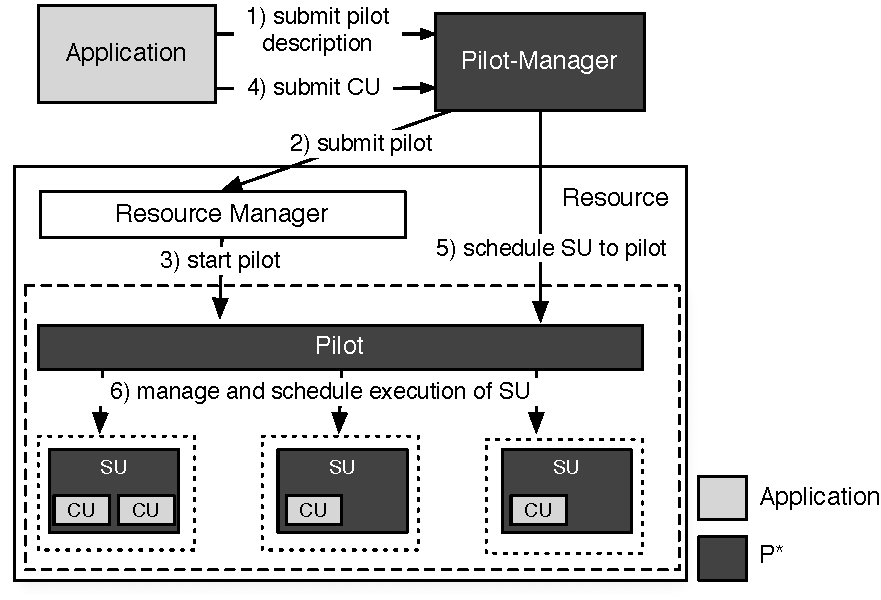
\includegraphics[width=0.4\textwidth]{figures/pstar_model_single.pdf}
    \caption{ \textbf{P* Model: Elements and
        Interactions:} The pilot manager (PM) is the central entity of a \pilot 
     framework. It has two functions: it manages 1) Pilots (step 1-3) and 2) the 
     execution of \cus.}
	\upp\upp
    \label{fig:figures_pstar}
\end{figure}


The Pilot-API is an {\it interoperable} and {\it extensible} API which
exposes the core functionalities of a \pilot framework via a unified
interface providing a common API that can be used across multiple
distinct production cyber infrastructures.  The API provides five
core classes: the \texttt{PilotComputeService} for the management of
Pilot-Jobs, \texttt{PilotDataService} for the management of Pilot-Data
and the \texttt{ComputeDataService} for the management of
\texttt{ComputeUnits} (CUs) and \texttt{DataUnits} (DUs). 
A CU represents a primary self-containing piece of work, while a DU
represents a logical set for data~\cite{pstar-2012}.

 
\subsection{BigJob: A \pilotcompute Implementation}

The abstraction of a {\emph \pilotjob} (PJ) generalizes the
reoccurring concept of utilizing a placeholder job as a container for
a set of compute tasks; instances of that placeholder job are commonly
referred to as Pilot-Jobs or pilots. The PJ provides application-
(user-) level control and management of the set of allocated resources.

BigJob (BJ) is a SAGA-based PJ framework that implements the Pilot-API. BJ has
been designed to be general-purpose and extensible. While BJ has been originally
built for HPC infrastructures, such as XSEDE and FutureGrid, it is generally
also usable in other environments, such as OSG. This extensibility mainly arises
from the usage of SAGA as a common API for accessing distributed resources.
% SAGA provides a simple, POSIX-style API to the most common
% grid functions at a sufficiently high-level of abstraction so as to be
% independent of the diverse and dynamic grid environments~\cite{pstar-2012}.

\subsection{BigData: A \pilotdata Implementation}

Analogous to \pilotjobs, {\it Pilot-Data} (PD) abstraction provides late-binding
capabilities for data by separating the storage allocation and application-level
\dataunits~\cite{pstar-2012}. For this purpose, the API defines the {\it
\pilotdata (PD)} and {\it \dataunit (DU)} entity: A \pd function as a
placeholder object that reserves storage spaces for a set of \dus.

\begin{figure}[t]
	\upp\upp
	\centering
		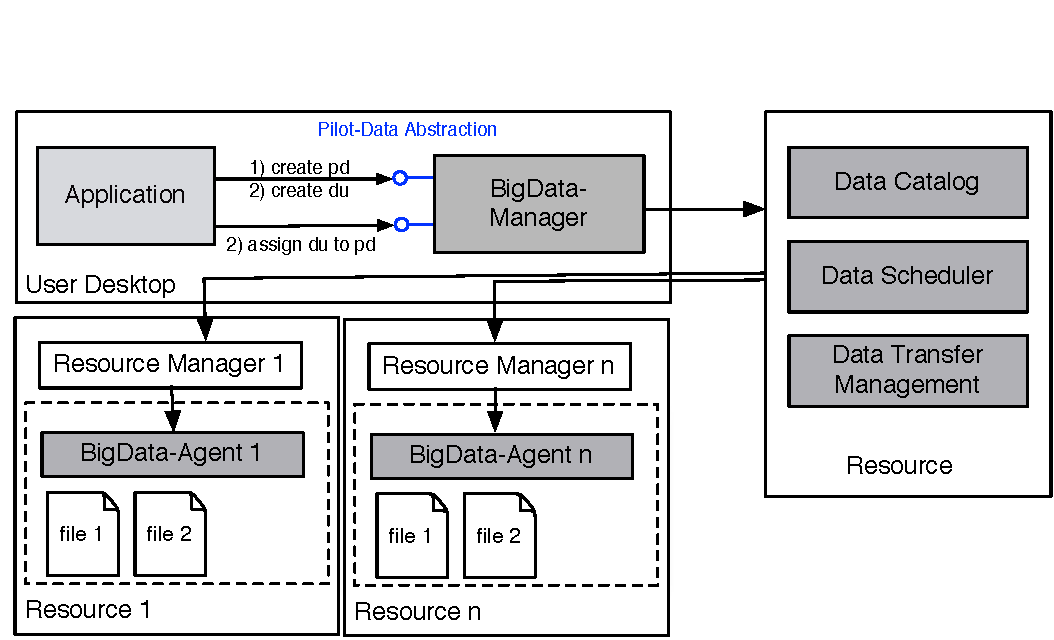
\includegraphics[width=0.4\textwidth]{figures/bigdata.pdf}
	\caption{BigData Architecture and Interactions\upp\upp\upp\upp\upp\upp}
	\label{fig:figures_bigdata}
\end{figure}

{\it BigData (BD)} is an implementation of the Pilot-Data
abstraction. BigData is designed as an extension of 
BigJob~\cite{bigjob_web} -- a SAGA-based Pilot-Job implementation.
Figure~\ref{fig:figures_bigdata} provides an overview of the
architecture of BigData. Similar to BigJob, it is comprised of two
components: the BD-Manager and the BD-Agents, which are deployed on
the physical resources.  The coordination scheme used is Master-Worker
(MW), with some decentralized intelligence located at the BD-Agent.
Analogous to BJ, the SAGA Advert Service~\cite{saga_advert} 
%\jhanote{not described or referenced} \alnote{fixed} 
provides a distributed communication mechanism in a push/pull mode.

The BD-Manager is responsible for (i) meta-data management, i.\,e.\ it
keeps track of all \pd and associated \dus, 
% \jhanote{pilot stores are undefined!?}\alnote{fixed}
(ii) for scheduling of data movements and replications 
(taking into account the application requirements defined
via affinities), and (iii) for managing data movements activities. 
BigData supports plug-able storage adaptors -- currently an adaptor 
for SSH, WebHDFS~\cite{webhdfs} and Globus Online~\cite{10.1109/MIC.2011.64}
is provided. 

% \jhanote{I think this paragraph should be zapped. (i) We have not
%   defined DU and CU yet. (ii) not do I see mention of a BD
%   Scheduler. This makes sense after a discussion of affinities} 
% \alnote{merged with affinity sub-section}

\upp
\subsection{Scheduling and Affinities}
\label{sec-affinities}

A critical requirement for data-intensive application, is the
management of compute and data dependencies, also referred to as {\it
  affinities}. The Pilot-API promotes affinities as a first class
characteristic for describing relationships between data and/or
compute supporting dynamic decision making.  Unfortunately, most
production infrastructure lack system-level support for affinities,
e.\,g.\ resource localities cannot be introspected. Data storage in
particular in distributed settings, such as in the XSEDE or the EGI
environment, is often a black box for the application with unknown
quality of services, i.e., the application usually does not know what
bandwidths and latencies it can expect. To address these deficiencies
the Pilot-API introduces affinities at the application-level:
applications can associate compute and data units with affinity
labels. The BigJob/BigData runtime ensures that CUs and DUs are placed
with respect to the affinity requirements.

The PMR framework assigns each file output from a map task to a reduce
partition. For each reduce partition, a DU containing the respective
files is created. Then, PMR submits the reduce CUs and DUs using the
Pilot-API. The affinity-aware scheduler assigns CUs and DUs to
appropriate resources taking into account data localities and
minimizing the amount of necessary data movements, i.\,e.\ if possible
a CU is always moved to a DU.  The Pilot-API and BigJob/BigData
provide an effective way to manage both compute and data units and the
relationships between them liberating the applications from the
challenging task of assigning/scheduling/managing Compute and
\dataunits.

%\secrev{ In introduction, it is mentioned that Pilot-API promotes
%  affinities as a first class characteristic for describing the
%  relationship between compute and data elements. However, the paper
%  misses to give the details about affinities, particularly about the
%  way they are computed, and the algorithm that assigns the CUs to DUs
%  based on the computed affinities.} \pnote{can we refer P* paper - if
%  not we need to describe the algorithm that assigns the CUs to DUs}
%\alnote{we have the ref. in there already. I added a sentence on }


%The BD scheduler is  affinity-aware: both BigJob and
%BigData are tightly integrated to efficiently support compute- and
%data-related aspects of dynamic execution.



\upp
\section{Pilot-MapReduce -- A Pilot-based MapReduce Implementation}
\label{sec-pilot-mr}
%\alnote{We should only use PilotMapReduce to refer to our framework - SAGA does not need to be in the name and mentioned all the time}

% \jhanote{Not sure why we have the first instanc of
%   ``\pilotmapreduce'' in ``\emph''. Also we toggle between PMR and
%   ``\pilotmapreduce''. Please be consistent} \alnote{ok removed
%   emph}
  

\pilotmapreduce (PMR) is a \pilot-based implementation of the
MapReduce programming model. 
% In PMR the actual management of the 
% compute, data and network resources are decoupled using \pilot-based
% abstractions.
By decoupling job scheduling and monitoring from the resource management using
\pilot-based abstraction, PMR can efficiently re-use the resource management
and late-binding capabilities of BigJob and BigData. PMR exposes an
easy-to-use interface, which provides the
% \jhanote{Need to
% talk about the following sentence/claim...} \alnote{yes, we should
% add some example code}
complete functionality needed by any MapReduce algorithm, while hiding
the more complex functionality, such as chunking of the input, sorting
the intermediate results, managing and coordinating the map \& reduce
tasks, etc., which are implemented by the framework.



%\alnote{Can we put a code snipped in here somewhere? maybe a separate sub-section}

%Pilot-API is used for managing map and reduce compute units
%and for defining relationships between the intermediate data and reduce tasks
%across distributed infrastructure

\upp
\subsection{Architecture of \pilotmapreduce}
\pilotmapreduce introduces a clean separation of concerns between
management of compute and data on the one hand, with their scheduling
in a distributed context. The pilot abstractions enable the easy
acquisition of both compute and storage resources. 
 
Figure~\ref{fig:figures_mapreduce-pilotdata} shows the architecture of
the \pilotmapreduce framework. PMR relies on BigJob to launch
MapReduce workers through a set of \pilots. The MR Workers are
responsible for running chunk, map and/or reduce tasks. \mrmg packages
data chunks into \dus and associates them with \pilotdata objects,
which are placed close to \pilotcomputes by BigData.  The \mrmg can
focus on orchestrating this resource pool.



\begin{figure}[t]
	\centering
	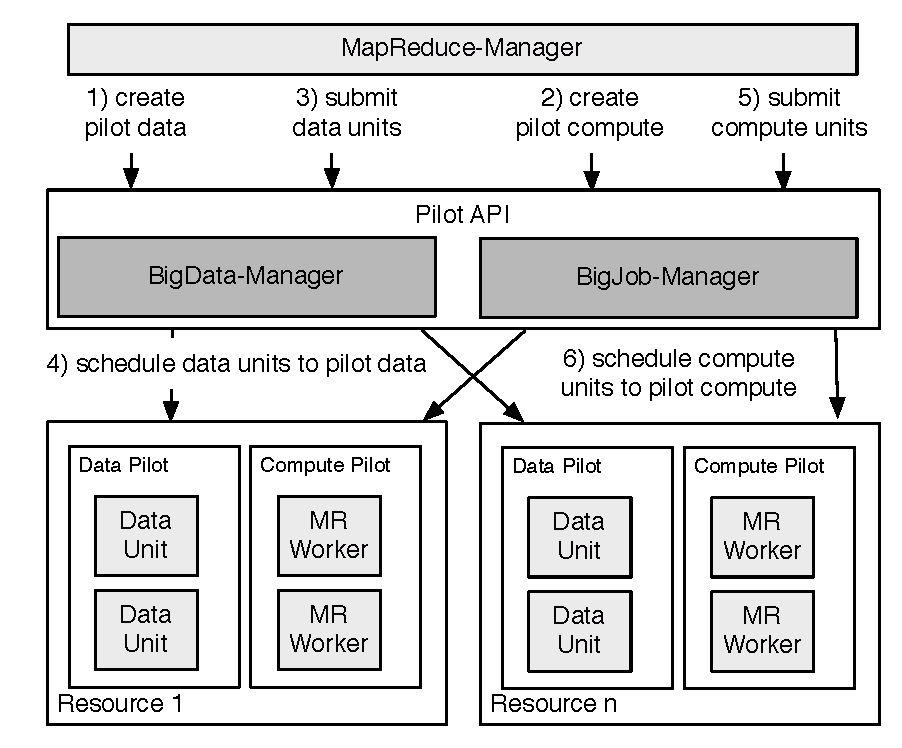
\includegraphics[width=0.38\textwidth]{figures/mr-arch.pdf}
	\caption{\textbf{Pilot-based MapReduce:} Each pilot (both compute and data 
	pilot) can be associated with an affinity label. The BigData and BigJob 
	Manager will ensure that CUs and DUs are placed with respect to these 
	requirements.\upp}
	\label{fig:figures_mapreduce-pilotdata}
\end{figure}

The flow of a typical MapReduce application involves the chunking of
the data, the execution of the map compute tasks, shuffling and moving
the intermediate data to the reduce task and finally the execution of
the reduce tasks.  \pilotmapreduce utilizes a set of compute and data
pilots for this application workflow:

% \jhanote{Worth noting that
%   these numbers don't correspond to the numbers in Figure 2, which in
%   of itself is not a problem, but we should try to make sure the
%   reader doesn't look to figure 2 to understand these
%   steps..}\alnote{changed enumeration list to A., B. referencing steps
%   in fig.}
\upp
\begin{compactenum}[A.]

\item Initially, the \mrmg allocates a set of compute and data
  resources by starting one (or most often a set of) compute and data
  pilots on different resources.  In general, on each resource one
  compute and one data pilot is co-located. The data pilot is either
  created with reference to local input data or the input data is
  moved to the data pilot after its creation.

%\pnote{Do we need data pilot initially? since we place the compute pilot on the resource where input data is present} 
%   \alnote{I think when we move to the distributed scenario this will
%     be the default flow, because we then also have to manage the input
%     data.}

\item \textbf{Chunking:} % \pnote{commented - The input data on each resource is
% {\it chunked}.}
  The \mrmg executes a \cu on each resource, which splits the input
  data on the respective resource with respect to the defined chunk
  size.\label{stp:chunking} % \alnote{how many chunking CUs are there? 1 per
% resource?}
Each chunk is stored in a new DU. BigJob and BigData -- in particular
the \texttt{ComputeDataService} -- are used as the common abstraction
for managing the \computeunits and \dataunits. 
  
  \jhanote{I'm not clear what ``executes a set of chunk compute
    units'' means? Plus the two previous sentence should be merged
    into 1 sentence?} \jhanote{I'm confused: isn't chunking all about
    data? why are we getting into executing CUs? shouldn't DUs be
    introduced in the chunking phase? currently no mention of DUs?}
  % \alnote{As mention above: I think we should describe the final
  %   scenario with distributed (and not) pre-staged input data}

\item \textbf{Mapping:} The \mrmg assigns a {\it map} CU to each
  chunk created in step~\ref{stp:chunking}. Again, BJ is used for
  managing the CUs. BJ and BD ensures that each CUs is co-located with
  an appropriate DU taking into account data localities and minimizing
  the amount of data movements. % \jhanote{there is no
% mention of DUs so far. Where/how does this happen?} \alnote{added DU
% creation part to chunk phase, so it should be clearer now.}  The
% execution of the map CUs is done analogous to the chunk CUs via
% BigJob.
\jhanote{Also,how are the chunks related to/assigned to DUs? that is
  unclear from description}\alnote{removed sentence. We were probably
  referring to the fact the the CU is executed via the pilot}
	
\item \textbf{Shuffling:} %\pnote{partitioning and sorting of
  % map output is part of map task}. \alnote{Hadoop Definitive Guide:
  % ``The process by which the system performs the sort and transfers
  % the map outputs to the reducers as inputs is known as the
  % shuffle.'' - I would prefer to work with this definition since it
  % encapsulates this intermediate step very well. Rather then
  % including it in the mapping phase (even if it might be done
  % partially by the mapper process.) } 
  After the map phase is completed the output data is sorted and
  partitioned. For each partition a \du is created. Each partition is
  then processed by a reduce task. For this purpose, the \mrmg assigns
  each reduce CU to a DU. Each DU comprises of a group of sorted,
  partitioned map output files. \cus and \dus are then submitted
  through the \texttt{ComputeDataService} of BJ and BD. The
  affinity-aware scheduler ensure that \cus are assigned to local \dus
  minimizing the amount of data transfers.  For each reduce task a
  Data Unit containing the necessary input files is created and
  submitted. % (step 3/4 in
  %figure~\ref{fig:figures_mapreduce-pilotdata})

\jhanote{shouldn't it
    be from the location of the map CUs to the location of the reduce
    CUs?} 
		
  % \alnote{We need to introduce what we mean by a distributed PMR.}
	
\item \textbf{Reducing:} The {\it reduce} tasks are prepared and
  executed on the DUs representing the intermediate data.
  % (step  5/6 in figure~\ref{fig:figures_mapreduce-pilotdata}).  
  The management of the data transfers is done by BJ/BD taking into account the 
  specified affinities.
	
\item The \pilots are terminated.

\end{compactenum}
\upp
% \jhanote{The mapping from the Chunking/Mapping/Shuffling stages to the
%   diagram steps is a bit hard to grasp. For example although we talk
%   about chunking, we find a mention of step 5/6..}
% \alnote{yes, since both aspects are a bit orthogonal. The figure shows
%   how compute and data units are managed via Pilot abstractions. The
%   phases are more about what the MR framework does in the CUs and
%   where DUs need to be moved. Should we remove the steps from the
%   enumeration?} \jhanote{Maybe remove the steps for now and if time
%   permits discuss them separately/lately?}
The PMR relies on the master/worker coordination model, i.\,e.\ a
central \mrmg orchestrates a set of MapReduce workers, which in turn
are responsible for executing map and reduce tasks. The \mrmg utilizes
BigJob and BigData, and in particular the central
\texttt{ComputeDataService} for executing mapper and reduce tasks.
This architecture can also efficiently support workloads that
currently not supported well enough by Hadoop, e.\,g.\ iterative
applications.

\upp
\subsection{Compute and Data Management}

The Pilot-API provides a well-defined interface for supporting the
late-binding of compute and data units decoupling resource assignment
from resource usage. Using BJ and BD, PMR can allocate both storage
and compute resources, which can then be flexibly utilized for
executing map and reduce tasks as well as for storing both
intermediate and output data.

The API also allows the expression and management of relationships
between data units and/or compute units.  BigJob and BigData provide
an implementation of the Pilot-API.  These frameworks ensure that the
data and compute affinity requirements of the MapReduce applications
are met for each step of the MapReduce workflow. For example, in the
shuffle phase for each reduce task a DU and CU is generated. These are
then submitted to BigJob and BigData framework, which handles the
scheduling, transfer of the DU and execution of the CU. PMR assigns a
resource affinity to each DU and CU. BJ and BD then ensure that each
CU is co-located to the right DU.


% (Listing~\ref{lst:pcs_creation}).

% \alnote{Can we do a MR specific example?}
% 
% \lstset{
% language=Python,
% frame=single,
% captionpos=b,
% stringstyle=\ttfamily,
% basicstyle=\scriptsize\ttfamily
% }
% \noindent\begin{minipage}{0.47 \textwidth}
% \begin{lstlisting}[caption={\textbf{Pilot Compute Creation:} Instantiation of a Pilot Job using Pilot Compute Description}, label={lst:pcs_creation}]
% pcs = PilotComputeService()
% cds = ComputeDataService()
% pjd ={"service_url":"pbs-ssh://sierra.futuregrid.org", 
% "number_of_processes": '8',
% "walltime":10, 
% "processes_per_node:'8',
% "affinity_datacenter_label":'sierra',
% "affinity_machine_label":'sierra'}
% pj=pcs.create_pilot(pilot_compute_description=pjd)
% cds.add_pilot_compute_service(pcs)
% \end{lstlisting}
% \end{minipage}

The efficiency of PMR  on multiple resources depends on
the management of the the intermediate data. BigData not only
provides flexibility to manage the relationship between data and
compute units, but also allows {\it parallel} data transfers between
machines and between data units.  BigData is used for moving the
intermediate output files of the mapper tasks to the resource where
the reduce compute units are executed.  

Interestingly, Hadoop also utilizes a job and task tracker: the job
tracker is the central manager that dispatches map and reduce tasks to
the nodes of the Hadoop cluster. On each node the task tracker is
responsible for executing the respective tasks. The main limitation of
this architecture is the fact that it intermixes both cluster resource
management and application-level task managements. Thus, it is not
easily possible to integrate Hadoop with another resource management
tool, e.\,g.\ PBS or Torque. Also, the job tracker represents a single
point of failure and scalability bottleneck.


\upp
\subsection{Distributed and Hierarchical MapReduce}
\label{sec:pmr-distributed}%  \jhanote{I propose we change this to Distributed and 
% Hierarchical MapReduce to be consistent with 5.4. ok?} \pnote { fine for me }

An increasing amount of data that scientific applications need to
operate on is distributed. Often data generation
and processing are far apart: For example, the Earth Science Grid
federates data of various climate simulations~\cite{ESG}. Meta-genomic
workflows need to process and analyze data generated by various
sequencing machines~\cite{Jha:2011fk}; the localization onto a single
resource is often not a possibility.

Several options for running Hadoop on distributed data have been
proposed~\cite{weissman-mr-11}: (i) in a global MapReduce setup one
central JobTracker and HDFS NameNode is used for managing a
distributed set of resources; (ii) in a hierarchical MapReduce setup
multiple MapReduce clusters are used: a MapReduce cluster close to the
data source for pre-processing data and a central cluster for
aggregating the different de-central data sources. The volume of the
pre-processed data is generally lower and thus, can be easily moved to
another processing resource. 

Ref~\cite{weissman-mr-11} shows that a hierarchical Hadoop
configuration leads to a better performance than a global Hadoop
cluster for some applications. A drawback of this approach is the
increased complexity: Hadoop is not designed with respect to a
federation of multiple MapReduce clusters. Setting up such a system
typically requires a lot of manual effort.


  

% BigJob and
% BigData will ensure that the affinity requirements of the MR framework
% are met. 
% \jhanote{The last sentence is a repitition}\alnote{removed}

\begin{figure}
	\upp
	\centering
	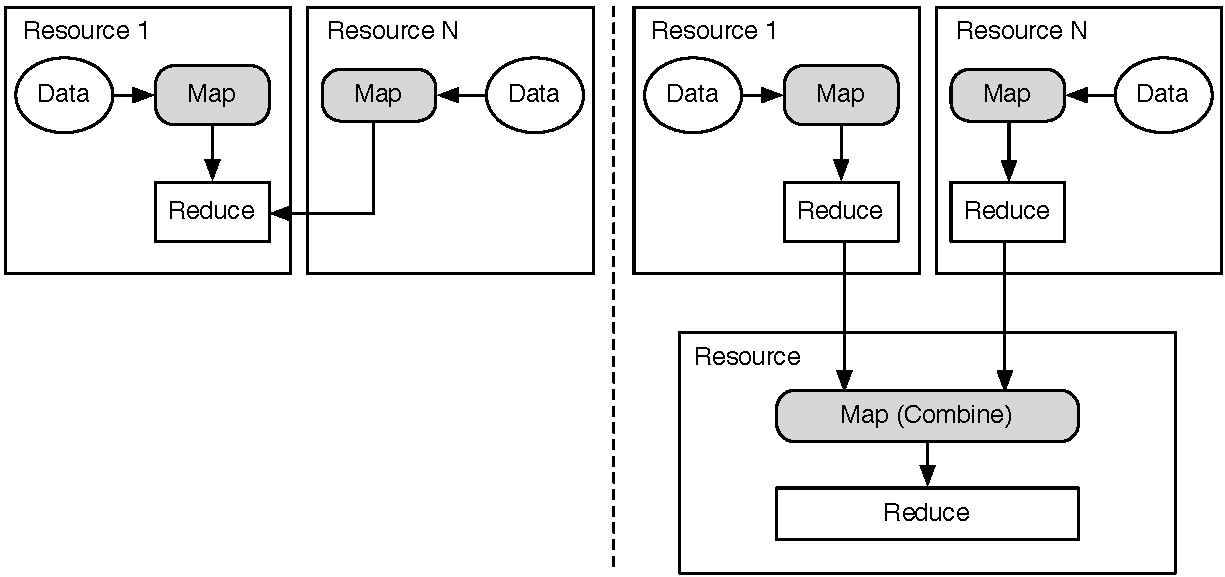
\includegraphics[width=0.42\textwidth]{figures/distributed_hierachical.pdf}
	% \label{fig:figures_distributed-mapreduce}}
%	\subfigure[Distributed PMR(implemented)]{
%		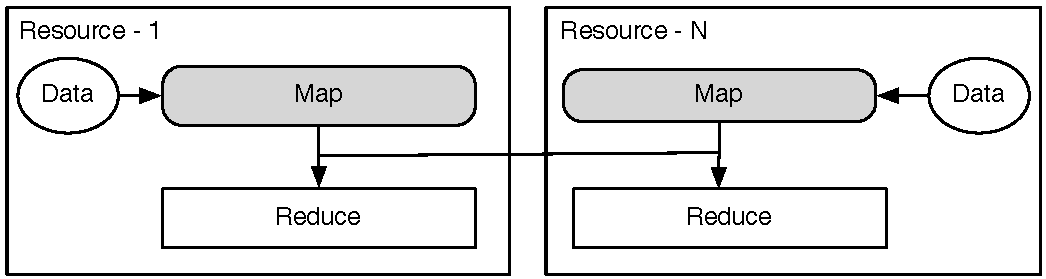
\includegraphics[width=0.4\textwidth]{figures/distributed_pmr_exchange.pdf}
%		\label{fig:figures_distributed-mapreduce-exchange}}
	% \subfigure[Hierachical PMR]{
	% 	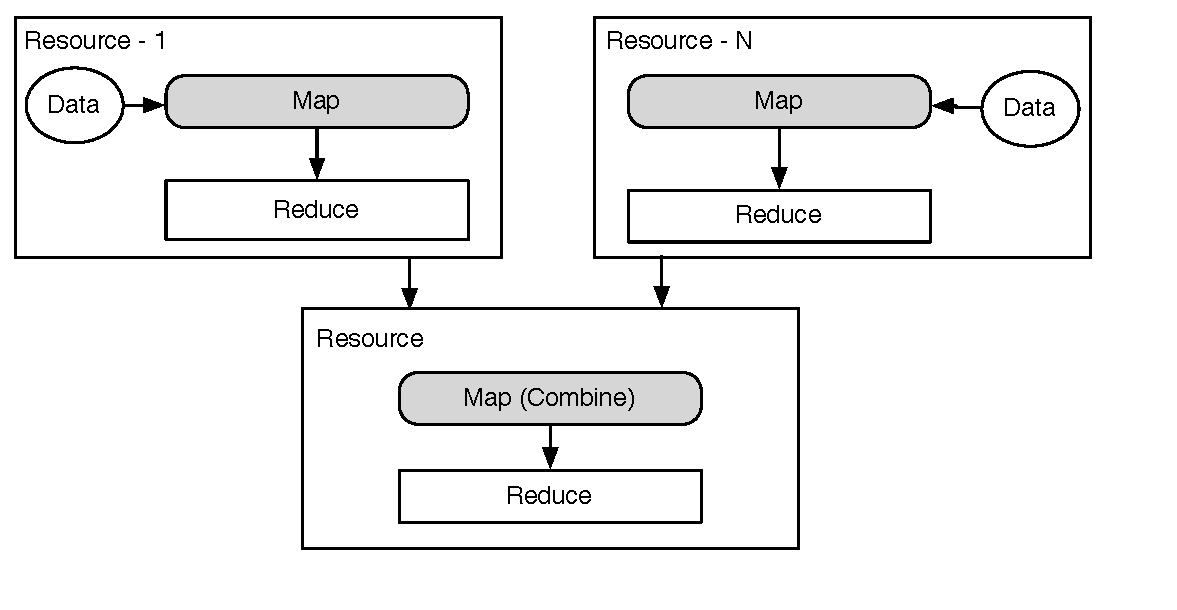
\includegraphics[width=0.4\textwidth]{figures/hierachical-mapreduce.pdf}
	%\label{fig:figures_hierachical-mapreduce}}
	\caption{\pilotmapreduce Deployment Scenarios: In the
          distributed scenario (left), the mapping tasks are run close
          to the data; reduced tasks are then run on a single
          resource. In the hierarchical scenario (right) two full
          MapReduce runs are
          conducted. \label{fid:distributed-mapreduce-overview}\upp\upp}
\end{figure}


\pilotmapreduce supports different distributed MapReduce topologies:
(i) \emph{local}, (ii) \emph{distributed} and (iii)
\emph{hierarchical}. A local PMR performs all map and reduce
computations on a single resource.
Figure~\ref{fid:distributed-mapreduce-overview} shows options (ii) and
(iii): A distributed PMR utilizes multiple resources often to run map
tasks close to the data to avoid costly data transfers; the
intermediate data is then moved to another resource for running the
reduce tasks. BigJob and BigData are used for managing CUs and DUs and
the necessary data movements. In contrast, in a hierarchical PMR the
outputs of the first complete MapReduce run are moved to a central
aggregation resource. A complete MapReduce run is then executed on
this resource to combine the results. % \jhanote{What about
%   Hierarchical: it can be distributed and/or local. Shouldnt
%   specify/discuss explicitly that it is not orthogonal to first two?}
% \alnote{for readability, I would then rather not refer to local at all
%   in this section. Also, while a local hierarchical MR is possible, it
%   doesn't really make sense, because the whole point is to reduce data
%   movement between resources. In a single cluster data needs to get
%   moved anyways.}


\pilotmapreduce uses the Pilot-API as an abstraction for compute and data
resources, as well as managing both \computeunits (i.\,e.\ map and reduce tasks)
and \dataunits. Using these abstractions, PMR can efficiently manage data and
compute localities and operate on a dynamic and distributed pool of storage and
compute resources. Using descriptive affinities label the data flow between CUs,
i.\,e.\ the transfer of the intermediate data, can be efficiently managed. Using
this capability PMR can be easily scaled out to multiple resources to support
scenarios (ii) and (iii).

%thus the Pilot-API provides a consistent API for managing

% A {\it distributed-PMR} provides an opportunity to utilize multiple
% distributed production infrastructure to run the map and reduce
% computations.  Therefore, the challenge to make use of multiple
% clusters to act collaboratively as one is addressed by
% distributed-PMR.

% \alnote{\textbf{place somewhere:} Unfortunately, users cannot
%   directly deploy a MapReduce framework such as Hadoop on top of
%   distributed production infrastructures to form a single larger
%   MapReduce cluster. Typically the internal nodes of a cluster are
%   not directly reachable from outside. However, MapReduce requires
%   the master node to directly communicate with any slave node, which
%   is also one of the reasons why MapReduce frameworks are usually
%   deployed within a single cluster. [hierarchical mapreduce
%   paper]. Hadoop is mainly designed for cluster/local environment,
%   but not for a high degree of distribution.}



% FROM Pradeep: should be covered in this section resp. perf section so # fare
% In ~\cite{weissman-mr-11}, different workload data aggregation schemes are
% evaluated. High Aggregation: The MapReduce output is multiple orders of
% magnitude smaller than the input, e.g. Wordcount on English plain-text. Zero
% Aggregation: The MapReduce output is the same size as the input, e.g. the Sort
% workload. There is no MapReduce configuration regarding low aggregation
% schemes, where the output data is significant and between high and zero
% aggregation schemes. In this experiment, we try to prove that \pilotmapreduce
% is a best model for low aggregation schema applications. We choose
% ~\cite{weissman-mr-11} DMR configuration and compare it with \pilotmapreduce
% with genome sequence application, which produces significant amount of output
% and neither high aggreation nor zero aggregation. We ran experiments with
% 20GB, 40GB and 80GB on two machines and 30GB, 60GB , 120GB on 3 machines.
\upp
\section{Experiments and Results}
\label{sec-experiments}


In this section we analyze the performance and scalability of
\pilotmapreduce and compare it to Hadoop MapReduce using different
applications. For this purpose we run several experiments on
FutureGrid (FG)~\cite{fg}. We run the experiment on the following FG
resources: India, Sierra and Hotel. Each experiment is repeated at
least three times. For our Hadoop experiments, we use Hadoop
0.20.2. At the begining of each run a Hadoop cluster is started via
the Torque resource management system on a specified number of
nodes. The first assigned node is used as master node running the
Hadoop JobTracker and the NameNode. The HDFS replication factor is set
to 2 and number of reduces to 8.  \upp
\subsection{MapReduce-Based Applications}

MapReduce has been utilized in various science applications. A key performance 
factor is the amount of data that must be moved through the MapReduce system. 
The degree of data aggregation of the map tasks is thus, an important 
characteristic of a MapReduce application~\cite{weissman-mr-11}.

MapReduce application can be classified with respect to different
criteria: (i) the volume of the intermediate data (i.\,e.\ the size of
the output of the map tasks), and (ii) the volume of the output data,
(i.\,e.\ the size of reduce phase output), and the relative proportion
of these data volume. In the following we investigate two application
scenarios: Word Count and a Genome Sequencing application.

% \jhanote{The following paragraph should move to next section. Also
%   need to explain the different axes of analysis: high vs low
%   aggregation between phases; local versus distributed; hierarchical
%   versus non-hierarchical. Currently all clobbered together and
%   difficult to read} 
% \alnote{\textbf{Incorporate:} }

% Computing widely distributed data using a traditional single cluster-MapReduce
% may not achieve an optimal MapReduce runtime. Several MapReduce configurations were
% proposed for distributed data processing based on the data
% aggregation~\cite{weissman-mr-11}. In high-data aggregation application the
% MapReduce output is multiple orders of magnitude smaller than input.
% Hierarchical MapReduce configuration is considered as an optimal choice since it
% involves less amount of output data to be transferred to the combine MapReduce
% phase. In zero or ballooning data aggregation applications, the intermediate and
% output data generated is larger than or equal to input data.  So, the all the input data from
% multiple clusters is moved to a single cluster, and then MapReduce job is performed, which is 
% known as Local MapReduce. Even though the initial data transfers are costly in case of Local-MapReduce \jhanote{this
% is a term; please define a term before using it}, they are needed
% because of lack of an abstraction which manages the relationships between the
% data and compute units effectively across wide-area systems. So, BigData optimizes runtime of \pilotmapreduce by allowing
% flexibility to specify intermediate data and reduce compute affinities, and required concurrent data movement between machines and data units.
%\upp
%\subsubsection*{Word Count}

{\it Word count:} The Word Count application is the basis for many machine
learning use cases, used e.\,g.\ for the classification of documents or
clustering. Word Count generates a large volume of intermediate data
($\sim$200$\%$). The volume of the output data depends on the type of input
data, e.\,g.\ the size of the output data is larger for a random input than for
an input in a natural language.

% \upp
% \subsubsection*{Genome Sequencing (GS)}

{\it Genome Sequencing (GS):} High-throughput genome sequencing as
provided by Next Generation Sequencing (NGS) platforms is changing biological
sciences and biomedical research. The data volumes generated by sequencing
machines is increasing rapidly. The distributed processing of this data requires
a sophisticated infrastructure. We utilize MapReduce to model
an important part of the sequencing workflow: the read alignment and the
duplicate removal. We use two implementations: the Hadoop-based
SEQAL~\cite{seal-2011} application and a PMR-based implementation 
GS/PMR. Both applications implement the read alignment in the mapping phase of
the application using BWA aligner~\cite{Li:2010:FAL:1741823.1741825}. In the
SEQAL case the duplicate removal in the reduce phase is implemented using
Picard's \texttt{rmdup}~\cite{picard}. 
% The GS/PMR reduce phase is not an exact implementation of SEQAL's Picard 
% \texttt{rmdup} implementation. We developed a custom
% script in python which is based on duplicate removal description provided in
% ~\cite{seal-2011}. 
The GS/PMR reducer removes duplicate reads based on the key
fields-chromosome, position and strand of the mapper output.

%%%%%%%%%%%%%%%%%%%%%%%%%%%%%%%%%%%%%%%%%%%%%%%%%%%%%%%%%%%%%%%%%%%%%%%%%%%%

\subsection{Characterizing Word Count}


In the first experiment, we benchmark the performance of
\pilotmapreduce and Hadoop using a simple Word Count application on a
single resource. For both frameworks, 8 nodes on India machine are
used. In all scenarios the input data is pre-staged on the respective
resources, i.\,e.\ for Hadoop the data is located in HDFS, for PMR the
data is stored on a shared file system. We set the total number of
reduces to 8 for both Hadoop and \pilotmapreduce; further, the default
chunk size of 128\,MB is used. A HDFS replication factor of 2 is used.

The runtime of PMR includes the time to chunk input data, running the
mapping CUs, shuffling (which in-turn comprises of sorting and the
intermediate data transfer), and finally running the reduce CUs.
Figure~\ref{fig:figures_wc_pmr_hmr} shows the results. The runtime of
Hadoop MapReduce includes the time to load input source data into HDFS and
MapReduce runtime.

\begin{figure}[ht]
	\centering
		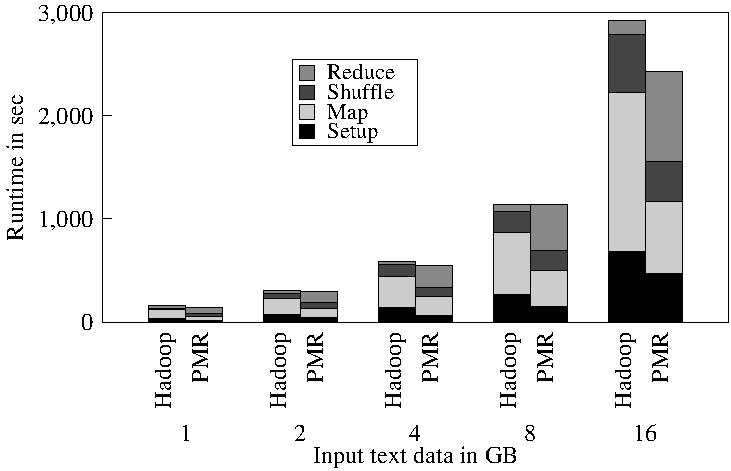
\includegraphics[width=0.47\textwidth]{figures/wc_pmr_hmr.pdf}
                \caption{PMR vs. Hadoop (Word Count): The performance
                  of Hadoop and PMR is comparable. The runtime 
                  increases with the input data size. Hadoop tasks
                  have a notable higher startup time.\upp}
\label{fig:figures_wc_pmr_hmr}
\end{figure}		
	
The time to solution increased linearly as data size increased; the performance
of both Hadoop and PMR is comparable up to 8\,GB. However, for the largest
volumes of input data we examined, PMR shows a better performance than Hadoop.
In particular, the setup, map and shuffle phase in the Hadoop case are longer.
Both the map and shuffle phase are the most data-intensive phases -- Word Count
needs to read all input files and generates intermediate data with the size of
about 200\,\% of the input data. Hadoop shows the worst shuffle performance. A
reason is that we were unfortunately not able to run HDFS in an optimal
configuration due to a lack of local storage on the FG machine. Thus, HDFS was
configured to utilize a shared file system.
%  PMR relies mostly on the shared
% file system for handling the intermediate data. 
% \jhanote{the last
%   statement is not obvious. It is confusing too.. because earlier we
%   talk about how PMR avoids bottlenecks traditionally associated with
%   Hadoop/HDFS}\alnote{rephrased}
  

% \jhanote{Can we say why?}\alnote{Pradeep: did we use the tmp directory
%   of the shared file system in the 16 GB case? Could be again a
%   sub-optimal Hadoop deployment.}\pnote{Yes- the /tmp directory of the
%   data node is pointed to a shared file system; as andre mentioned,
%   the map phase involves huge amounts of data(nearly 200\%) to be
%   written to the disk.}

% \alnote{Not sure whether we should mention these - these issues are
%   well-known: Observed performance issues: 1) HDFS performs better
%   when nodes local data directory is used.. But performance degrades
%   if shared storage is used.  2) when a single node is used to launch
%   all workers, hadoop fails with lot of memory problems, whereas PMR
%   successfully completed all tasks.  reasons for this problem}

%http://tech.backtype.com/the-dark-side-of-hadoop+J204		
\upp\upp
\subsection{Characterizing Genome Sequencing}

In this section, we compare and contrast GS/PMR and SEQAL. For both
applications, we utilize the same input data comprising of different
sizes of read files and the reference genome. SEQAL, however, expects
the input data in a different format (\texttt{prq} instead of
\texttt{fastq}); data was converted to meet the SEQAL
requirements. For GS/PMR, the \texttt{fastq}
files from sequencing machines are directly used; further, a custom
chunk script is used to chunk the \texttt{fastq} files based on the number of
reads. The chunk size for both SEQAL and PMR are equal. For both
GS/PMR and SEQAL, a total of 4 nodes on FG Sierra machine, 8
reduces, 2 workers/node, default chunk size of 128\,MB is used. For
Hadoop based SEQAL, the replication factor of two is used.  
% Since
% SEQAL and GS/PMR utilize different duplicate removal tools in the
% reduce phase, we focus our investigation on the map phase.

%  to compare scalability of PMR across clusters, we are
% interested in only in the execution of map phase. SEQAL provides an option to
% turnoff the reduce phase and just perform the map phase. For PMR a custom 
% mapper
% script is developed in Python, which uses core BWA aligner. 

\begin{figure}[ht]
	\centering
		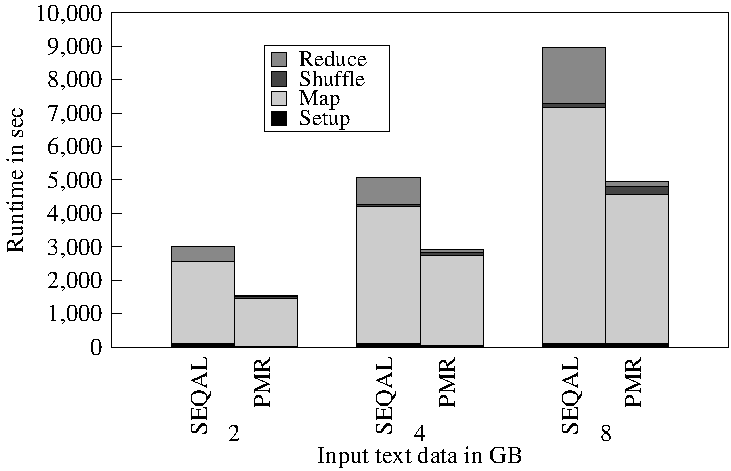
\includegraphics[width=0.47\textwidth]{figures/gs_seq_pmr.pdf}
\caption{SEQAL and GS/PMR: GS/PMR provides a marginal better
  performance that SEQAL. The overhead of SEQAL is mainly attributed
  to the usage of shared file system for HDFS.\upp}
% \jhanote{needs fixing: double ``used''}\upp }
% \pnote{addressed}
\label{fig:gs_seq_pmr}
\end{figure}		

Figure~\ref{fig:gs_seq_pmr} shows the comparative results of both
SEQAL and GS/PMR applications. The time required to copy and extract
the reference genome to HDFS is included in the SEQAL set-up time. In
comparison to Word Count GS applications are more compute intensive,
i.\,e.\ the ratio between computation in the map phase and the size of
the input data is significantly larger. Furthermore, SEQAL has a larger
time-to-completion than GS/PMR. Both the map and reduce phase of SEQAL
are longer. While the map phase of SEQAL relies on the same BWA
implementation as GS/PMR, the reduce phase uses Picard's
\texttt{rmdump}~\cite{picard} for duplicate removal, which has a
significant longer runtime than the duplicate removal process in the
reduce phase of GS/PMR.
% \jhanote{We just said above that we will focus on the map
%   phase after stating that the reduce phases are different. So why are
%   we now discussing reduce phases?}  \jhanote{Also not sure How/why
%   the previous follow from subsequent sentence?} \alnote{removed the
%   sentence that states that we focus on the reduce phase. Would
%   propose to analyze and explain the data in the figure which
%   incl. the reduce phase. Will remove redundancies.}  \jhanote{Andre
%   to fix} 
A reason for the slower runtime of SEQAL in the map phase is the non-optimal
Hadoop configuration: As described, the local disks available on FG are too
small; thus, HDFS had to be configured to utilize a shared, distributed file
system, which leads to a non-optimal performance during the I/O intensive map
phase.

% The difference in the reduce phase
% mainly originate from the different implementations of the duplicate
% removal process in SEQAL and GS/PMR. \jhanote{this is a repeat of an
%   earlier statement! No details of reduce phase in GS/PMR provided!}

% \jhanote{Is the following for the Map phase or true for all phases?}
% \alnote{added sentence on analysis of both phases} \alnote{Pradeep:
%   Please elaborate a bit on the differences} \upp\upp \jhanote{AL to
%   clear up all of 5.3}
\upp
\subsection{Characterizing Distributed and Hierarchical MapReduce}

% \jhanote{I changed the title of this subsection. Please confirm if OK}
% \pnote{fine for me}

In this section, we evaluate the performance and scalability of the (i)
distributed and (ii) hierarchical PMR configuration using the Word Count
application on natural language and on random data as well as the genome
sequencing application. In the distributed PMR scenario, the CUs are
distributed across two machines; in the hierarchical PMR two resources are used,
each executing an independent MR run. The MapReduce run for combining and
aggregating the output of the first round is executed on one of these machines.
The performance of each application depends on the amount of generated
intermediate and output data. Table~\ref{tab:data-volumes} summarizes the
characteristics of the used applications.

\begin{table}[ht]
	\centering
\begin{tabular}{|p{2cm}|c|c|c|}
\hline
\textbf{Application} &\textbf{Input} &\textbf{Intermediate} &\textbf{Output}\\
\hline
GS/PMR 		&80\,GB &71\,GB		 &17\,GB\\
\hline
Word Count\linebreak[4] (English) &16\,GB&26\,GB&20\,MB\\
\hline
Word Count (random) &16\,GB&30\,GB&30\,GB\\
\hline
\end{tabular}
\caption{Data Volumes for different Applications\upp\upp}
\label{tab:data-volumes}
\end{table}

\upp\upp
\subsubsection*{Word Count}

For Word Count we compare a distributed and hierarchical PMR
configuration with the performance of two Hadoop configurations: a
single resource Hadoop configuration and a hierarchical Hadoop setup
with two resources. We utilize two machines, Sierra and Hotel. For all
configurations, we use 8 nodes. The initial input data of 16\,GB is
equally distributed on these two machines. For the single resource
Hadoop configuration, half of the input data needs to be moved from
Sierra to Hotel prior to running the actual MapReduce
job. Unfortunately, the FG firewall rules prohibited the usage
of a distributed Hadoop setup.

Figure~\ref{fig:allmrs_rands} shows the results. For natural language
input, both Hadoop and PMR show comparable performance. A major
determinant of performance for Hadoop (in the case of distributed
data) is the necessity to move parts of the data (half of the input
data) to the central Hadoop cluster. The performance of PMR is
determined by the runtime of the map and reduce phase, which are
slightly longer than for Hadoop mainly due to the resource
heterogeneity and the resulting scheduling overhead: the slowest node
determines the overall runtime of both the map and reduce phase.

Both hierarchical Hadoop and PMR perform better than
the distributed PMR and single resource Hadoop configuration. The
performance is mainly influenced by data movement costs. In the
distributed PMR scenario, half of the {\it intermediate} data needs to
be moved to the other resource; in the hierarchical case half of the
{\it output} data requires movement. Since the output data in the
hierarchical case is a magnitude smaller than the intermediate data in
the distributed case (cmp. table~\ref{tab:data-volumes}) -- 20\,MB in
cmp. to 30\,GB -- the performance in the hierarchical case is
significantly better.

%  implementations, since they involves very less amount of output data generated
% and involves less combine overhead. Hadoop suffers the initial data transfer of
% 8GB from Sierra to Hotel and HDFS load times. In case of distributed PMR the
% intermediate data 12.85\,GB moved using Pilot-Data resulting in a effective data
% transfer of 1.6\,GB. The data transfer and amount to reduce the entire
% intermediate data results in higher runtime of distributed PMR.

For random data, the distributed PMR and single resource Hadoop
perform better than the hierarchical PMR and hierarchical Hadoop
configuration. As the output data is approximately equal to the
intermediate data (30\,GB), i.\,e.\ the advantage of a reduced
transfer volume does not exit. For random data, the additional
MapReduce run represents an overhead. In the Hadoop case, the moved
data needs to be loaded into HDFS, which represents another overhead.

% since it moves only required data in the intermediate phase and
% there are no initial or combine outputs overhead. The intermediate data that
% needs to be moved from Sierra to Hotel is 15.45\,GB, and data related to each
% reduce nearly 1.9\,GB is segregated as data unit. The Pilot-Data supports
% parallel transfer of data units, which results in an effective data transfer of
% 1.9\,GB This leads to the performance of distributed PMR. Hadoop suffers the
% initial data transfer of 8\,GB from Sierra to Hotel and HDFS load times. In
% hierarchical Hadoop, we transferred the total output reduce data 14.8\,GB using
% Pilot-Data, where each data unit consists a reduce output file. So that all
% reduces can be transferred in parallel and effective data transfer would be
% nearly 1.85\,GB. But loading 14.8\,GB on Hotel contributed significantly towards its
% the entire runtime. Hierarchical PMR is closer to distributed PMR, but it
% involves combine MapReduce overhead.
% In the random setup, a hierarchical 
% setup cannot be recommended since the amount of data that needs to be moved is 
% not lower than in the distributed case.

% In general, the distributed PMR has an advantage over the hierarchical PMR if
% the intermediate data is small (such as in the natural language case). If the
% data is distributed, the performance of Hadoop is impacted by the time necessary
% to move the input files to the single Hadoop resource.


\begin{figure}[t]
	\upp
	\centering
		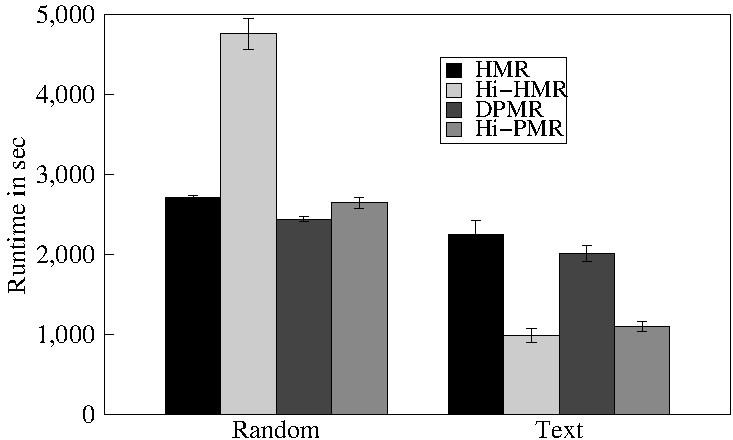
\includegraphics[width=0.47\textwidth]{figures/allmrs_rands.pdf}
\caption{Word Count on 16\,GB Data Using Hadoop, Hierarchical Hadoop, Distributed PMR  and Hierarchical PMR} 	
\label{fig:allmrs_rands}
\end{figure}		

\upp\upp
\subsubsection*{Genome Sequencing}

\begin{figure}[t]
	\centering
		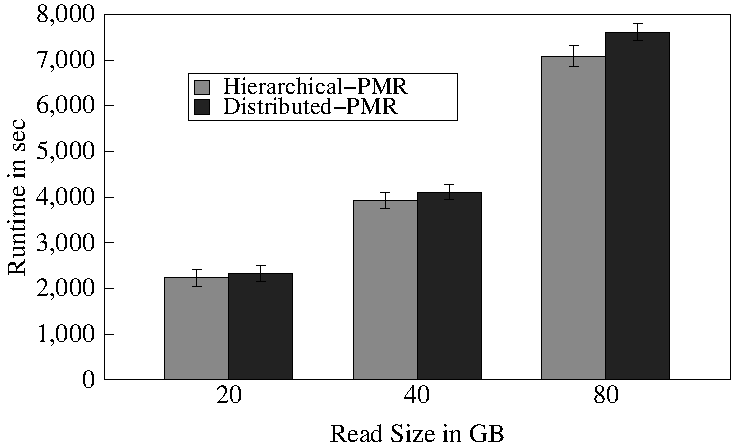
\includegraphics[width=0.47\textwidth]{figures/gs_hihmr_dpmr.pdf}
                \caption{Time to completion of GS/PMR for 20, 40 and
                  80GB using Hierarchical and Distributed PMR. These
                  measurements were performed utilizing a total of 32
                  nodes on India and Hotel. \upp\upp\upp}
\label{fig:gs_hihmr_dpmr}
\end{figure}		

For the genome sequencing application, we investigate hierarchical and
distributed PMR scenarios utilizing a total of 32 nodes on India and
Hotel. We vary the input data size between 20 and 80\,GB.
Figure~\ref{fig:gs_hihmr_dpmr} shows the results. In both scenarios
the runtime increases with the input data size. For the distributed
PMR, a significant part of the performance is determined by the
movement of the intermediate data -- 71\,GB for the 80\,GB problem set
(see table~\ref{tab:data-volumes}). In the hierarchical PMR scenario,
the main overhead arises from the additional MapReduce run. For GS/PMR
the hierarchical configuration shows a slight advantage over the
distributed setup, since the amount of data that needs to be
transferred is significant less: half of the output, i.\,e.\ 8.5\,GB,
respectively, of the intermediate data, i.\,e.\ 36\,GB. However, a
great amount of the time saved in the transfer is offset by the
overhead of the additional MapReduce run.

% \begin{table}[h]
% \begin{tabular}{|l|c|c|c|c|}
% \hline
% \textbf{MapReduce} &\textbf{Data to be moved} &\textbf{Effective 
% data transfer}&\textbf{Parallel transfers}\\
% \hline
% HMR  &8\,GB &8\,GB		 &1\\
% \hline
% Hi-HMR &14.8\,GB&1.85\,GB&8\\
% \hline
% DPMR&15.45\,GB&1.93\,GB&8\\
% \hline
% Hi-PMR&15.20\,GB&1.9\,GB&8\\
% \hline
% \end{tabular}
% \caption{Data Volumes for Word Count application with 16GB random data}
% \label{tab:data-volumes-random}
% \alnote{Pradeep: please fill out}
% \end{table}
% 
% 
% 
% \begin{table}[h]
% \begin{tabular}{|l|c|c|c|c|}
% \hline
% \textbf{MapReduce} &\textbf{Data to be moved} &\textbf{Effective 
% data movement}&\textbf{Parallel transfers}\\
% \hline
% HMR  &8\,GB &8\,GB		 &1\\
% \hline
% Hi-HMR &16\,MB&2\,MB&8\\
% \hline
% DPMR&12.85\,GB&1.6\,GB&8\\
% \hline
% Hi-PMR&16\,MB&2\,MB&8\\
% \hline
% \end{tabular}
% \caption{Data Volumes for Word Count application with 16GB natural langauge text data}
% \label{tab:data-volumes-text}
% \alnote{Pradeep: please fill out}
% \end{table}
% 
% \begin{table*}[h]
% \begin{tabular}{|l|c|c|c|c|}
% \hline
% \textbf{MapReduce} &\textbf{Read size} &\textbf{Data to be moved} &\textbf{Effective 
% data transfer}&\textbf{Parallel transfers}\\
% \hline
% Hi-HMR &20\,GB&3.04\,GB&0.38\,GB&8\\
% \hline
% DPMR &20\,GB&9.32\,GB&1.22\,GB&8\\
% \hline
% 
% \hline
% Hi-HMR &40\,GB&5.79\,GB&0.724\,GB&8\\
% \hline
% DPMR &40\,GB&18.46\,GB&2.42\,GB&8\\
% \hline
% 
% \hline
% Hi-HMR &80\,GB&8.73\,GB&1.09\,GB&8\\
% \hline
% DPMR &80\,GB&35.6\,GB&\,4.45GB&8\\
% \hline
% 
% \end{tabular}
% \caption{Data Volumes for Genome Sequencing application}
% \label{tab:data-volumes-gs}
% \alnote{Pradeep: please fill out}
% \end{table*}
% A correlation exists between the input data sizes and the
% performance of MapReduce configurations.  Analysis

In summary, optimizing MapReduce for distributed data is not a trivial
task: 
% the overall performance is determined by many factors, e.\,g.\
% the application's characteristics, current machine and network loads,
% etc. 
% The distributed and
% hierarchical configuration, can be used to support certain application
% characteristics. 
Depending on the volumes of the intermediate and output data, a distributed or
hierarchical configuration may have better performance. In applications with a
less output volume compared to intermediate data, such as GS and Word Count on
natural languages, a hierarchical MapReduce is a good choice since it involves
less data movement. PMR provides the flexibility to deploy MapReduce workloads
in different configurations optimizing the performance with respect to the
characteristics of different applications. Hadoop, in contrast, is very
inflexible in supporting different kind of MapReduce configurations, due to
deployment challenges (e.\,g.\ we were not able to run Hadoop across more than
two machines on FG due to firewall issues) as well as runtime limitations.

% \alnote{\textbf{For Analysis:} In distributed-PMR on m clusters with n
%   reduces distributed evenly across clusters involve n*(m-1) parallel
%   data transfers to complete the intermediate data movement. Thus
%   BigData play a major role in reducing the runtime of a
%   distributed-PMR running on multiple clusters.  } 
\upp\upp
\section{Discussion and Future Work}
\label{sec-conclusion}

\pilotmapreduce provides a flexible runtime environment for MapReduce
applications on general-purpose distributed infrastructures, such as XSEDE and
FutureGrid. It brings the advantages of the Pilot abstraction to MapReduce, and
enables utilization of federated and heterogeneous compute and data resources.
In contrast to Hadoop, no previous cluster setup, which includes running several
Hadoop/HDFS daemons, is required. Pilot-MapReduce provides a extensible runtime
environment, which allows the flexible usage of sorting in the shuffle, more
fine-grained control of data localities and transfer, as well as support for
different MapReduce topologies. Using these capabilities, applications with
different characteristics, e.\,g.\ compute/IO and data aggregation ratios, can
be efficiently supported. 

%Pilot-Abstractions and affinities are a powerful tool

The Pilot abstraction, and specific the BigJob and BigData
implementation have proven to be a powerful tool for developing
PMR. Using finer-grain affinity specifications for compute/data units
and resources, the runtime is able to optimize compute and data
placement as well as transfers. These capabilities are essential for
PMR, especially when dealing with large amounts of distributed data;
in order to achieve an optimal performance in this case the
application must be able to reason and trade-off properties, such as
data/compute localities and data transfers to achieve an optimal
performance.

Moving forward, we will extend the capabilities of PMR and BigData to
support use cases, such as data streaming, data caching as well as
different data/compute scheduling heuristics. Further, we will explore
scenarios and applications with dynamic data and execution. An obvious
and trivial extension will be to implement Iterative MapReduce using
PMR. A clear advantage will be to obviate the need to distinguish
between static and dynamic data, for PMR will be able to treat both
symmetrically.  \upp

% \jhanote{I know space is tight but we should also consider reminding
%   the reader about in the conclusion, why the PMR approach (especially
%   in the case of HMR) is better than a shared file system approach...
%   For example, I quote from Judy's paper on
%   HMR~\cite{ecmls11-mr-autodock}: `` There are two weaknesses in the
%   Gfarm solution. First, the Gfarm file system in the cross-cluster
%   sense only accesses the front nodes of clusters. If there is no
%   shared file system in a local cluster, the storage of Gfarm is
%   limited. Secondly, although in most of the cases, a cluster has its
%   own shared file system, the following weakness still hold. Since
%   Gfarm and HDFS use separate directories on the front node of each
%   cluster, the data copy operation between Gfarm file system and HDFS
%   is unavoidable in our implementation.''  i.e., PMR is not only
%   elegant from an abstraction point of view but also from an
%   engineering and deployment point of view. Thoughts?}



% The following two commands are all you need in the
% initial runs of your .tex file to
% produce the bibliography for the citations in your paper.
\bibliographystyle{abbrv}
%\bibliographystyle{unsrt}
\bibliography{pilotjob,saga,saga-related,mrbib}  % sigproc.bib is the name of the Bibliography in this case
% You must have a proper ".bib" file
%  and remember to run:
% latex bibtex latex latex
% to resolve all references
%
% ACM needs 'a single self-contained file'!
%

\upp
\subsection*{Acknowledgments}
\scriptsize This work is funded by NSF CHE-1125332 (Cyber-enabled
Discovery and Innovation), HPCOPS NSF-OCI 0710874 award, NSF-ExTENCI
(OCI-1007115) and NIH Grant Number P20RR016456 from the NIH National
Center For Research Resources. Important funding for SAGA has been
provided by the UK EPSRC grant number GR/D0766171/1 (via OMII-UK) and
the Cybertools project (PI Jha) NS-F/LEQSF (2007-10)-CyberRII-01. SJ
acknowledges the e-Science Institute, Edinburgh for supporting the
research themes: Distributed Programming Abstractions \& 3DPAS. SJ 
acknowledges useful related discussions with Jon Weissman (Minnesota)
and Dan Katz (Chicago). We thank J Kim (CCT) for assistance with
genome sequencing application. This work has been made possible
thanks to resources provided by TeraGrid TRAC award
TG-MCB090174 (Jha). This document was developed with support from the
US NSF under Grant No. 0910812 to Indiana University for FutureGrid.
\end{document}
